\subsubsection{Decommissioning}		 
The following use cases pertain to the decomissioning of Condenser components. Figure~\ref{DecomissioningUse} shows a diagram depicting the relationships between the decomissioning use cases.
\begin{center}
	\begin{figure}[htbp]
		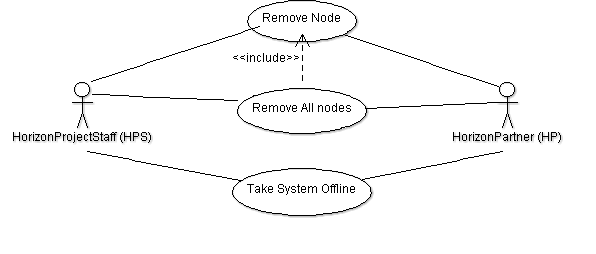
\includegraphics[scale=.5]{images/DecomissioningUse.png}
		\caption{Use cases defining Condenser decomissioning.\label{DecomissioningUse}}
	\end{figure}
\end{center}	

	Removing a node \\	 
	\textbf{Participating Actors:}  ... \\
	\textbf{Event Flow:}
	\begin{enumerate}
\item  ...
    \end{enumerate}
	\textbf{Entry Conditions:}\\
	\textbf{Exit Conditions:}\\
	\textbf{Quality Requirements:}\\
	\line(1,0){350}		

	Removing all nodes \\	 
	\textbf{Participating Actors:}  ... \\
	\textbf{Event Flow:}
	\begin{enumerate}
\item  ...
    \end{enumerate}
	\textbf{Entry Conditions:}\\
	\textbf{Exit Conditions:}\\
	\textbf{Quality Requirements:}\\
	\line(1,0){350}		

	Taking Condenser offline \\	 
	\textbf{Participating Actors:}  ... \\
	\textbf{Event Flow:}
	\begin{enumerate}
\item  ...
    \end{enumerate}
	\textbf{Entry Conditions:}\\
	\textbf{Exit Conditions:}\\
	\textbf{Quality Requirements:}\\
	\line(1,0){350}		